% ==================================================================
%  §7.5  n 元函数的连续与极限
%  源：徐森林、薛春华《数学分析》第二册，印刷页 40-51 (PDF p. 46-57)
%  底本：PaddleOCR-VL-1.6 JSON/MD 识别结果，人工逐字核校与公式精修
%  规范：全西文标点，忠实原文定义、注、定理、例题、练习题编号与推导
% ==================================================================

\section{$n$ 元函数的连续与极限}\label{sec:7.5}

设 $A \subset \mathbb{R}^{n}$, $f\colon A \to \mathbb{R}^{1}$ 为 $n$ 元函数,
\[
  x = (x_{1}, x_{2}, \cdots, x_{n}) \mapsto y = f(x) = f(x_{1}, x_{2}, \cdots, x_{n}) \in \mathbb{R}^{1}.
\]

\begin{definition}\label{def:7.5.1}
设 $A \subset \mathbb{R}^{n}$, $x^{0} \in \overline{A}$. 如果 $\forall \varepsilon > 0$, $\exists \delta > 0$, 当 $x \in A$, 且 $0 < \|x - x^{0}\| < \delta$ 时, 有
\[
  |f(x) - l| < \varepsilon,
\]
则称 $f$ 当 $x$ (在 $A$ 中或沿 $A$) 趋于 $x^{0}$ 时, 有极限 $l$, 记作
\[
  \lim_{x \to x^{0}} f(x) = l,
\]
或
\[
  \lim_{(x_{1}, x_{2}, \cdots, x_{n}) \to (x_{1}^{0}, x_{2}^{0}, \cdots, x_{n}^{0})} f(x_{1}, x_{2}, \cdots, x_{n}) = l,
\]
或
\[
  \lim_{\substack{x_{1} \to x_{1}^{0} \\ x_{2} \to x_{2}^{0} \\ \vdots \\ x_{n} \to x_{n}^{0}}} f(x_{1}, x_{2}, \cdots, x_{n}) = l.
\]
此极限也常称为 \textbf{$n$ 重极限}.
\end{definition}

\begin{remark}\label{rem:7.5.1}
从\cref{def:7.5.1} 可知,
\[
  \lim_{\substack{x \to x^{0} \\ x \in A}} f(x) = l \iff \lim_{\substack{x \to x^{0} \\ x \in B}} f(x) = l,\ \forall B \subset A.
\]
因此, 如果有 $B \subset A$, 使得
\[
  \lim_{\substack{x \to x^{0} \\ x \in B}} f(x)
\]
不存在, 或者有 $B_{1} \subset A$, $B_{2} \subset A$, 使得
\[
  \lim_{\substack{x \to x^{0} \\ x \in B_{1}}} f(x) = l_{1} \neq l_{2} = \lim_{\substack{x \to x^{0} \\ x \in B_{2}}} f(x),
\]
则
\[
  \lim_{x \to x^{0},\ x \in A} f(x)
\]
不存在.

特别考虑二元函数的二重极限, 有
\[
  \lim_{\substack{x \to x_{0} \\ y \to y_{0}}} f(x, y) = \lim_{(x, y) \to (x_{0}, y_{0})} f(x, y).
\]
二元函数还可考虑两个累次极限
\[
  \lim_{y \to y_{0}} \lim_{x \to x_{0}} f(x, y) \quad \text{与} \quad \lim_{x \to x_{0}} \lim_{y \to y_{0}} f(x, y).
\]
类似\cref{def:7.5.1} 可定义
\[
  \lim_{x \to x_{0}} f(x) = +\infty\ (-\infty\ \text{或}\ \infty),
\]
\[
  \lim_{\substack{x_{1} \to x_{1}^{0} \\ x_{2} \to x_{2}^{0} \\ \vdots \\ x_{n} \to \infty}} f(x) = l\ (+\infty, -\infty\ \text{或}\ \infty).
\]
\end{remark}

\begin{theorem}\label{thm:7.5.1}
设 $X \times Y \subset \mathbb{R}^{2}$, $x_{0} \in X'$, $y_{0} \in Y'$ (故 $(x_{0}, y_{0}) \in (X \times Y)'$), $f\colon X \times Y \to \mathbb{R}^{1}$ 为二元函数, 如果二重极限
\[
  \lim_{\substack{x \to x_{0} \\ y \to y_{0}}} f(x, y) = l\ (\text{实数}, +\infty, -\infty, \infty),
\]
且 $\forall y \in Y$ ($\forall x \in X$), 单重极限 $\lim\limits_{x \to x_{0}} f(x, y)$ $\left(\lim\limits_{y \to y_{0}} f(x, y)\right)$ 存在, 则累次极限
\[
  \lim_{y \to y_{0}} \lim_{x \to x_{0}} f(x, y) = l \quad \left(\lim_{x \to x_{0}} \lim_{y \to y_{0}} f(x, y) = l\right).
\]
\end{theorem}

\begin{proof}
只对 $l \in \mathbb{R}$ 加以证明, 其他读者自证.

因为 $\lim\limits_{\substack{x \to x_{0} \\ y \to y_{0}}} f(x, y) = l$, 所以 $\forall \varepsilon > 0$, $\exists \delta > 0$, 当 $x \in X$, $y \in Y$, $0 < |x - x_{0}| < \delta$, $0 < |y - y_{0}| < \delta$ (它等价于 $0 < \|(x, y) - (x_{0}, y_{0})\| < \delta$) 时, 有
\[
  |f(x, y) - l| < \frac{\varepsilon}{2},
\]
固定 $y$, $0 < |y - y_{0}| < \delta$, 令 $x \to x_{0}$ 得到
\[
  \left|\lim_{x \to x_{0}} f(x, y) - l\right| = \lim_{x \to x_{0}} |f(x, y) - l| \leqslant \frac{\varepsilon}{2} < \varepsilon.
\]
所以,
\[
  \lim_{y \to y_{0}} \lim_{x \to x_{0}} f(x, y) = l.\qedhere
\]
\end{proof}

类似讨论, 有 $\lim\limits_{\substack{x \to +\infty \\ y \to y_{0}}} f(x, y)$, $\lim\limits_{\substack{x \to \infty \\ y \to y_{0}}} f(x, y)$ 等定理.

对 $n$ 元函数 $f(x_{1}, x_{2}, \cdots, x_{n})$ 也有 $n$ 重极限及累次极限的概念, 且有相同的结果. 与一元函数一样, $n$ 元函数的极限有惟一性定理. 如果 $f$, $g$ 有有限极限, 则
\[
\begin{aligned}
  &\lim_{x \to x^{0}} (f \pm g)(x) = \lim_{x \to x^{0}} f(x) \pm \lim_{x \to x^{0}} g(x), \\
  &\lim_{x \to x^{0}} (fg)(x) = \lim_{x \to x^{0}} f(x) \cdot \lim_{x \to x^{0}} g(x), \quad \lim_{x \to x^{0}} (cf)(x) = c \lim_{x \to x^{0}} f(x), \\
  &\lim_{x \to x^{0}} \frac{f}{g}(x) = \frac{\lim\limits_{x \to x^{0}} f(x)}{\lim\limits_{x \to x^{0}} g(x)} \quad (\text{当}\ \lim_{x \to x^{0}} g(x) \neq 0\ \text{时}),
\end{aligned}
\]
其中 $c \in \mathbb{R}$. 其他类型的极限有相同的结果.

根据\cref{def:7.2.1} 可知, $f$ 在 $x^{0}$ 连续等价于 $\lim\limits_{x \to x^{0}} f(x) = f(x^{0})$, 即 $\forall \varepsilon > 0$, $\exists \delta > 0$, 当 $x \in A$, 且 $\|x - x^{0}\| < \delta$ 时, 有
\[
  |f(x) - f(x^{0})| < \varepsilon.
\]

\begin{theorem}\label{thm:7.5.2}
设 $A \subset \mathbb{R}^{n}$, $x^{0} \in A$, $f$ 与 $g$ 在 $x^{0}$ 均连续. 则 $f \pm g$, $fg$, $cf$ ($c \in \mathbb{R}$), $\dfrac{f}{g}$ ($g(x^{0}) \neq 0$) 也都在 $x^{0}$ 连续.
\end{theorem}

\begin{proof}
因 $\lim\limits_{x \to x^{0}} (fg)(x) = \lim\limits_{x \to x^{0}} f(x) \cdot \lim\limits_{x \to x^{0}} g(x) = f(x^{0})g(x^{0}) = (fg)(x^{0})$, 故 $fg$ 在 $x^{0}$ 连续. 其他类似证明.
\end{proof}

关于 $n$ 元函数还有很多概念, 方法, 定理的论述与一元函数相类似, 如归结原则, 夹逼定理, 连续函数的保号性与保不等式性等, 不再一一赘述.

\begin{example}\label{ex:7.5.1}
设函数 $f(x, y) = \dfrac{x^{2}y^{2}}{x^{2} + y^{2}}$, $(x, y) \neq (0, 0)$. 求 $\lim\limits_{\substack{x \to 0 \\ y \to 0}} f(x, y)$.
\end{example}

\begin{solution}
$\forall \varepsilon > 0$, 取 $\delta = \sqrt{2\varepsilon}$, 当 $0 < \|(x, y) - (0, 0)\| = \|(x, y)\| = \sqrt{x^{2} + y^{2}} < \delta$ 时,
\[
  \left|\frac{x^{2}y^{2}}{x^{2} + y^{2}} - 0\right|
  \left\{
  \begin{array}{ll}
    \leqslant \dfrac{x^{2}y^{2}}{2|xy|}, & x \neq 0,\ y \neq 0, \\[2.5mm]
    = 0, & x = 0,\ y \neq 0\ \text{或}\ y = 0,\ x \neq 0
  \end{array}
  \right.
\]
又有
\[
  \frac{x^{2}y^{2}}{2|xy|} = \frac{1}{2}|x||y| < \frac{\delta^{2}}{2} = \varepsilon,
\]
所以,
\[
  \lim_{\substack{x \to 0 \\ y \to 0}} \frac{x^{2}y^{2}}{x^{2} + y^{2}} = 0.\qedhere
\]
\end{solution}

\begin{example}\label{ex:7.5.2}
求二重极限 $\lim\limits_{\substack{x \to +\infty \\ y \to +\infty}} xye^{-x^{2}y^{4}}$.
\end{example}

\begin{solution}
$\forall \varepsilon > 0$, 取 $\Delta = \sqrt[4]{\dfrac{1}{\varepsilon}}$, 当 $x > \Delta$, $y > \Delta$ 时, 有
\[
  \left|xye^{-x^{2}y^{4}} - 0\right| = \frac{|xy|}{e^{x^{2}y^{4}}} \leqslant \frac{|xy|}{x^{2}y^{4}} = \frac{1}{|x||y|^{3}} < \frac{1}{\Delta^{4}} = \varepsilon,
\]
所以,
\[
  \lim_{\substack{x \to +\infty \\ y \to +\infty}} xye^{-x^{2}y^{4}} = 0.\qedhere
\]
\end{solution}

\begin{example}\label{ex:7.5.3}
求二重极限:
\begin{enumerate}
  \item $\lim\limits_{\substack{x \to 0 \\ y \to 0}} x^{2}\ln(x^{2} + y^{2})$;
  \item $\lim\limits_{\substack{x \to 0 \\ y \to 0}} x\ln(x^{2} + y^{2})$.
\end{enumerate}
\end{example}

\begin{solution}
(1) 因为 $\left|\dfrac{x^{2}}{x^{2} + y^{2}}\right| \leqslant 1$, 且
\[
  \lim_{u \to 0^{+}} u\ln u = \lim_{u \to 0^{+}} \frac{-\ln\frac{1}{u}}{\frac{1}{u}} = -\lim_{v \to +\infty} \frac{\ln v}{v} = -\lim_{v \to +\infty} \frac{\frac{1}{v}}{1} = 0,
\]
所以 $\lim\limits_{\substack{x \to 0 \\ y \to 0}} (x^{2} + y^{2})\ln(x^{2} + y^{2}) = 0$, 从而
\[
  \lim_{\substack{x \to 0 \\ y \to 0}} x^{2}\ln(x^{2} + y^{2}) = \lim_{\substack{x \to 0 \\ y \to 0}} \frac{x^{2}}{x^{2} + y^{2}}(x^{2} + y^{2})\ln(x^{2} + y^{2}) = 0.
\]
(2) $\lim\limits_{\substack{x \to 0 \\ y \to 0}} x\ln(x^{2} + y^{2}) = 2\lim\limits_{\substack{x \to 0 \\ y \to 0}} \dfrac{x}{\sqrt{x^{2} + y^{2}}} \sqrt{x^{2} + y^{2}} \ln\sqrt{x^{2} + y^{2}} = 0$.
\end{solution}

\begin{example}\label{ex:7.5.4}
求二重极限 $\lim\limits_{\substack{x \to 0 \\ y \to 0}} y\sin\dfrac{1}{x}$ 及累次极限 $\lim\limits_{y \to 0} \lim\limits_{x \to 0} y\sin\dfrac{1}{x}$, $\lim\limits_{x \to 0} \lim\limits_{y \to 0} y\sin\dfrac{1}{x}$.
\end{example}

\begin{solution}
$\forall \varepsilon > 0$, 取 $\delta = \varepsilon$, 当 $0 < \|(x, y) - (0, 0)\| = \sqrt{x^{2} + y^{2}} < \delta$ 时, 有
\[
  \left|y\sin\frac{1}{x} - 0\right| = \left|y\sin\frac{1}{x}\right| \leqslant |y| \leqslant \sqrt{x^{2} + y^{2}} < \delta = \varepsilon,
\]
所以二重极限
\[
  \lim_{\substack{x \to 0 \\ y \to 0}} y\sin\frac{1}{x} = 0.
\]
由于当 $y \neq 0$ 时, $\lim\limits_{x \to 0} y\sin\dfrac{1}{x}$ 不存在, 故累次极限 $\lim\limits_{y \to 0} \lim\limits_{x \to 0} y\sin\dfrac{1}{x}$ 不存在. 而 $\lim\limits_{y \to 0} y\sin\dfrac{1}{x} = 0$, 故
\[
  \lim_{x \to 0} \lim_{y \to 0} y\sin\frac{1}{x} = \lim_{x \to 0} 0 = 0 = \lim_{\substack{x \to 0 \\ y \to 0}} y\sin\frac{1}{x}.\qedhere
\]
\end{solution}

\begin{example}\label{ex:7.5.5}
证明: 二重极限 $\lim\limits_{\substack{x \to 0 \\ y \to 0}} \dfrac{xy}{x^{2} + y^{2}}$ 不存在.
\end{example}

\begin{proof}
令 $y = kx$, 则
\[
  \lim_{\substack{x \to 0 \\ y = kx \to 0}} \frac{xy}{x^{2} + y^{2}} = \lim_{x \to 0} \frac{kx^{2}}{x^{2} + k^{2}x^{2}} = \lim_{x \to 0} \frac{k}{1 + k^{2}} = \frac{k}{1 + k^{2}}.
\]
从上式可看出, $(x, y)$ 沿过 $(0, 0)$ 的斜率为 $k$ 的不同直线方向趋于 $(0, 0)$ 时, 极限值 $\dfrac{k}{1 + k^{2}}$ 各不相同, 根据归结原则知, 二重极限 $\lim\limits_{\substack{x \to 0 \\ y \to 0}} \dfrac{xy}{x^{2} + y^{2}}$ 不存在.

但是, 两个累次极限都存在且为 $0$.
\[
  \lim_{y \to 0} \lim_{x \to 0} \frac{xy}{x^{2} + y^{2}} = \lim_{y \to 0} \frac{0 \cdot y}{0 + y^{2}} = \lim_{y \to 0} 0 = 0,
\]
\[
  \lim_{x \to 0} \lim_{y \to 0} \frac{xy}{x^{2} + y^{2}} = \lim_{x \to 0} \frac{x \cdot 0}{x^{2} + 0} = \lim_{x \to 0} 0 = 0.\qedhere
\]
\end{proof}

\begin{example}\label{ex:7.5.6}
研究函数
\[
  f(x, y) =
  \begin{cases}
    \dfrac{x^{2}y}{x^{4} + y^{2}}, & (x, y) \neq (0, 0), \\[2.5mm]
    0, & (x, y) = (0, 0)
  \end{cases}
\]
在点 $(0, 0)$ 处的二重极限与累次极限. 并说明 $f(x, y)$ 沿每条过原点 $(0, 0)$ 的直线是连续的, 但此函数在点 $(0, 0)$ 并非连续.
\end{example}

\begin{solution}
先求两个累次极限:
\begin{align*}
  \lim_{y \to 0} \lim_{x \to 0} \frac{x^{2}y}{x^{4} + y^{2}} &= \lim_{y \to 0} \frac{0 \cdot y}{0 + y^{2}} = \lim_{y \to 0} 0 = 0, \\
  \lim_{x \to 0} \lim_{y \to 0} \frac{x^{2}y}{x^{4} + y^{2}} &= \lim_{x \to 0} \frac{x^{2} \cdot 0}{x^{4} + 0} = \lim_{x \to 0} 0 = 0.
\end{align*}
再来观察二重极限. 当 $(x, y)$ 沿直线 $y = kx$ 趋于 $(0, 0)$ 时,
\[
  \lim_{\substack{x \to 0 \\ y = kx \to 0}} \frac{x^{2}y}{x^{4} + y^{2}} = \lim_{x \to 0} \frac{x^{2} \cdot kx}{x^{4} + k^{2}x^{2}} = \lim_{x \to 0} \frac{kx}{x^{2} + k^{2}} = 0 = f(0, 0),
\]
由此还不能断定二重极限存在且为 $0$, 事实上, 当 $(x, y)$ 沿抛物线 $y = x^{2}$ 趋于 $(0, 0)$ 时,
\[
  \lim_{\substack{x \to 0 \\ y = x^{2} \to 0}} \frac{x^{2}y}{x^{4} + y^{2}} = \lim_{x \to 0} \frac{x^{4}}{x^{4} + x^{4}} = \lim_{x \to 0} \frac{1}{2} = \frac{1}{2} \neq 0 = \lim_{\substack{x \to 0 \\ y = kx \to 0}} \frac{x^{2}y}{x^{4} + y^{2}},
\]
由此可知二重极限 $\lim\limits_{\substack{x \to 0 \\ y = x^{2} \to 0}} \dfrac{x^{2}y}{x^{4} + y^{2}}$ 不存在. 因而, $f(x, y)$ 在 $(0, 0)$ 不连续.\qedhere
\end{solution}

\begin{example}\label{ex:7.5.7}
{\emergencystretch=4em
求二重极限 $\lim\limits_{\substack{x \to 0 \\ y \to 0}} \dfrac{x - y + x^{2} + y^{2}}{x + y}$ 及累次极限 $\lim\limits_{x \to 0} \lim\limits_{y \to 0} \dfrac{x - y + x^{2} + y^{2}}{x + y}$, $\lim\limits_{y \to 0} \lim\limits_{x \to 0} \dfrac{x - y + x^{2} + y^{2}}{x + y}$.\par}
\end{example}

\begin{solution}[解法 1]
因为
\begin{align*}
  \lim_{y \to 0} \lim_{x \to 0} \frac{x - y + x^{2} + y^{2}}{x + y} &= \lim_{y \to 0} \frac{-y + y^{2}}{y} = \lim_{y \to 0} (-1 + y) = -1 + 0 = -1, \\
  \lim_{x \to 0} \lim_{y \to 0} \frac{x - y + x^{2} + y^{2}}{x + y} &= \lim_{x \to 0} \frac{x + x^{2}}{x} = \lim_{x \to 0} (1 + x) = 1 + 0 = 1,
\end{align*}
所以
\[
  \lim_{y \to 0} \lim_{x \to 0} \frac{x - y + x^{2} + y^{2}}{x + y} \neq \lim_{x \to 0} \lim_{y \to 0} \frac{x - y + x^{2} + y^{2}}{x + y}.
\]
应用反证法及\cref{thm:7.5.1} 可知, $\lim\limits_{\substack{x \to 0 \\ y \to 0}} \dfrac{x - y + x^{2} + y^{2}}{x + y}$ 不存在.\noqedhere
\end{solution}

\begin{solution}[解法 2]
因为
\begin{align*}
  \lim_{(x, 0) \to (0, 0)} \frac{x - y + x^{2} + y^{2}}{x + y} &= \lim_{(x, 0) \to (0, 0)} \frac{x + x^{2}}{x} = \lim_{(x, 0) \to (0, 0)} (1 + x) = 1 + 0 = 1, \\
  \lim_{(0, y) \to (0, 0)} \frac{x - y + x^{2} + y^{2}}{x + y} &= \lim_{(0, y) \to (0, 0)} \frac{-y + y^{2}}{y} = \lim_{(0, y) \to (0, 0)} (-1 + y) = -1 + 0 = -1,
\end{align*}
所以
\[
  \lim_{(x, 0) \to (0, 0)} \frac{x - y + x^{2} + y^{2}}{x + y} \neq \lim_{(0, y) \to (0, 0)} \frac{x - y + x^{2} + y^{2}}{x + y}.
\]
根据\cref{rem:7.5.1} 推得 $\lim\limits_{\substack{x \to 0 \\ y \to 0}} \dfrac{x - y + x^{2} + y^{2}}{x + y}$ 不存在.\noqedhere
\end{solution}

\begin{solution}[解法 3]
因为当 $k \neq -1$ 时,
\begin{align*}
  \lim_{\substack{(x, y) \to (0, 0) \\ y = kx}} \frac{x - y + x^{2} + y^{2}}{x + y} &= \lim_{x \to 0} \frac{x - kx + x^{2} + k^{2}x^{2}}{x + kx} \\
  &= \lim_{x \to 0} \frac{1 - k + x + k^{2}x}{1 + k} = \frac{1 - k}{1 + k},
\end{align*}
故当 $k$ 不同时, 上述极限不同, 从而根据\cref{rem:7.5.1} 推得 $\lim\limits_{\substack{x \to 0 \\ y \to 0}} \dfrac{x - y + x^{2} + y^{2}}{x + y}$ 不存在.
\end{solution}

\begin{example}\label{ex:7.5.8}
设
\[
  f(x, y) = \frac{1}{2x^{2} + 3y^{2}},
\]
证明: $\lim\limits_{(x, y) \to (0, 0)} f(x, y) = +\infty$.
\end{example}

\begin{proof}
$\forall A > 0$, 取 $0 < \delta < \dfrac{1}{2\sqrt{A}}$, 当 $0 < \sqrt{x^{2} + y^{2}} = \sqrt{(x - 0)^{2} + (y - 0)^{2}} < \delta$ 时,
\[
  \frac{1}{2x^{2} + 3y^{2}} \geqslant \frac{1}{4(x^{2} + y^{2})} > \frac{1}{4\delta^{2}} > A,
\]
所以,
\[
  \lim_{(x, y) \to (0, 0)} f(x, y) = \lim_{(x, y) \to (0, 0)} \frac{1}{2x^{2} + 3y^{2}} = +\infty.\qedhere
\]
\end{proof}

\begin{example}\label{ex:7.5.9}
讨论函数 $f(x, y, z) = \sin(xy + z)$ 的连续性.
\end{example}

\begin{solution}
由定义知, $x$, $y$, $z$, $\sin u$ 都是连续函数, 而加, 减, 乘, 除运算及复合都保持连续性, 所以, $f(x, y, z) = \sin(xy + z)$ 在 $\mathbb{R}^{3}$ 中连续.
\end{solution}

\begin{example}\label{ex:7.5.10}
证明: 关于 $x$, $y$ 的有理函数
\[
  f(x, y) = \frac{xy}{x^{2} + y^{2}}, \quad (x, y) \neq (0, 0)
\]
在其定义域上连续, 但非一致连续.
\end{example}

\begin{proof}
从定义知, $x$, $y$ 连续. 再由 $f(x, y)$ 是由 $x$, $y$ 通过三次乘法, 一次加法, 一次除法而得到的, 而加, 减, 乘, 除运算保持连续性推得 $f(x, y)$ 在其定义域中连续.

取点列 $p_{n} = \left(\dfrac{1}{n}, \dfrac{1}{n}\right)$, $q_{n} = \left(\dfrac{1}{n}, 0\right)$, 则
\begin{align*}
  \rho_{0}^{2}(p_{n}, q_{n}) &= \|p_{n} - q_{n}\| = \left\|\left(\frac{1}{n}, \frac{1}{n}\right) - \left(\frac{1}{n}, 0\right)\right\| \\
  &= \left\|\left(0, \frac{1}{n}\right)\right\| = \frac{1}{n} \to 0 \quad (n \to +\infty),
\end{align*}
但
\[
  |f(p_{n}) - f(q_{n})| = \left|\frac{\frac{1}{n} \cdot \frac{1}{n}}{\left(\frac{1}{n}\right)^{2} + \left(\frac{1}{n}\right)^{2}} - \frac{\frac{1}{n} \cdot 0}{\left(\frac{1}{n}\right)^{2} + 0^{2}}\right| = \frac{1}{2} \neq 0 \quad (n \to +\infty).
\]
再应用反证法可知 $f$ 在其定义域上非一致连续.\qedhere
\end{proof}

如果二元函数 $f(x, y)$ 在点 $(x_{0}, y_{0})$ 连续, 由定义, 显然两个边缘函数 $f(x, y_{0})$, $f(x_{0}, y)$ 分别在 $x_{0}$, $y_{0}$ 处连续, 然而, 反之不真.

\begin{example}\label{ex:7.5.11}
设
\[
  f(x, y) =
  \begin{cases}
    \dfrac{xy}{x^{2} + y^{2}}, & (x, y) \neq (0, 0), \\[2.5mm]
    0, & (x, y) = (0, 0).
  \end{cases}
\]
因为
\[
  \lim_{x \to 0} f(x, 0) = \lim_{x \to 0} \frac{x \cdot 0}{x^{2} + 0} = \lim_{x \to 0} 0 = 0 = f(0, 0),
\]
\[
  \lim_{y \to 0} f(0, y) = \lim_{y \to 0} \frac{0 \cdot y}{0 + y^{2}} = \lim_{y \to 0} 0 = 0 = f(0, 0),
\]
所以两个边缘函数 $f(x, 0)$ 与 $f(0, y)$ 分别在 $x_{0} = 0$ 与 $y_{0} = 0$ 处连续, 此外, 根据\cref{ex:7.5.10} 知 $f(x, y)$ 在 $\mathbb{R}^{2} \setminus \{(0, 0)\}$ 中每一点都连续, 因此两个边缘函数 $f(x, y_{0})$, $f(x_{0}, y)$ 分别在 $x_{0}$, $y_{0}$ 处连续. 但是, 当 $k \neq 0$ 时, 因为
\[
  \lim_{\substack{x \to 0 \\ y = kx \to 0}} \frac{xy}{x^{2} + y^{2}} = \lim_{x \to 0} \frac{x \cdot kx}{x^{2} + k^{2}x^{2}} = \lim_{x \to 0} \frac{k}{1 + k^{2}} = \frac{k}{1 + k^{2}} \neq 0 = f(0, 0).
\]
所以 $f(x, y)$ 在 $(0, 0)$ 处不连续.\qedhere
\end{example}

\begin{exblock}{练习题 7.5}
  \item 确定并画出下列二元函数的定义域:

  \begin{tabular}{@{}p{0.45\linewidth}p{0.50\linewidth}@{}}
    (1) $u = x + \sqrt{y}$; & (2) $u = \sqrt{1 - x^{2}} + \sqrt{y^{2} - 1}$; \\
    (3) $u = \sqrt{x^{2} + y^{2} - 1}$; & (4) $u = \sqrt{1 - (x^{2} + y^{2})}$; \\
    (5) $u = \arcsin\dfrac{y}{x}$; & (6) $u = \ln(x + y)$; \\
    (7) $u = f(x, y) = \sqrt{x}$; & (8) $u = \arccos\dfrac{x}{x + y}$; \\
    (9) $u = \dfrac{x^{2} + y^{2}}{x^{2} - y^{2}}$; & (10) $u = \dfrac{1}{2x^{2} + 3y^{2}}$; \\
    (11) $u = \sqrt{xy}$; & (12) $u = \sqrt{\sin(x^{2} + y^{2})}$.
  \end{tabular}

  \item 确定下列三元函数的定义域, 并几何地描述它们:

  \begin{tabular}{@{}p{0.45\linewidth}p{0.50\linewidth}@{}}
    (1) $u = \ln(xyz)$; & (2) $u = \ln\sqrt{2 - (x^{2} + y^{2} + z^{2})}$; \\
    (3) $u = f(x, y, z) = \dfrac{1}{x^{2} + y^{2}}$; & (4) $u = \arccos\dfrac{z}{\sqrt{x^{2} + y^{2}}}$;
  \end{tabular}
  (5) $u = \sqrt{R^{2} - (x^{2} + y^{2} + z^{2})} + \dfrac{1}{\sqrt{x^{2} + y^{2} + z^{2} - r^{2}}}$, $R > r > 0$.

  \item 计算下列二重极限:

  \begin{tabular}{@{}p{0.45\linewidth}p{0.50\linewidth}@{}}
    (1) $\lim\limits_{(x, y) \to (0, 0)} \dfrac{\sin(xy)}{x}$; & (2) $\lim\limits_{\substack{x \to +\infty \\ y \to +\infty}} (x^{2} + y^{2})^{-(x + y)}$; \\[3mm]
    (3) $\lim\limits_{(x, y) \to (1, 0)} \dfrac{\ln(x + e^{y})}{\sqrt{x^{2} + y^{2}}}$; & (4) $\lim\limits_{\substack{x \to +\infty \\ y \to +\infty}} \left(\dfrac{xy}{x^{2} + y^{2}}\right)^{x^{2}}$; \\[3mm]
    (5) $\lim\limits_{\substack{x \to \infty \\ y \to \infty}} \dfrac{x + y}{x^{2} - xy + y^{2}}$; & (6) $\lim\limits_{(x, y) \to (0, 0)} (x^{2} + y^{2})^{x^{2}y^{4}}$; \\[3mm]
    (7) $\lim\limits_{(x, y) \to (+\infty, 0)} \left(1 + \dfrac{1}{x}\right)^{\frac{x^{2}}{x + y}}$; & (8) $\lim\limits_{(x, y) \to (+\infty, +\infty)} \left(1 + \dfrac{1}{xy}\right)^{x\sin y}$; \\[3mm]
    (9) $\lim\limits_{(x, y) \to (+\infty, +\infty)} (x^{2} + y^{2})e^{-(x + y)}$; & (10) $\lim\limits_{(x, y) \to (+\infty, +\infty)} \dfrac{x^{2} + y^{2}}{x^{4} + y^{4}}$.
  \end{tabular}

  \item 计算两个累次极限:
  \begin{enumerate}
    \item $\lim\limits_{x \to \infty} \lim\limits_{y \to \infty} \sin\dfrac{\pi x}{2x + y}$; \quad $\lim\limits_{y \to \infty} \lim\limits_{x \to \infty} \sin\dfrac{\pi x}{2x + y}$;
    \item $\lim\limits_{x \to +\infty} \lim\limits_{y \to 0^{+}} \dfrac{x^{y}}{1 + x^{y}}$; \quad $\lim\limits_{y \to 0^{+}} \lim\limits_{x \to +\infty} \dfrac{x^{y}}{1 + x^{y}}$.
  \end{enumerate}

  \item (1) 设
  \[
    f(x, y) = (x + y)\sin\frac{1}{x}\sin\frac{1}{y},
  \]
  证明: $f$ 在原点 $(0, 0)$ 处的两个累次极限均不存在, 但二重极限
  \[
    \lim_{(x, y) \to (0, 0)} f(x, y) = 0.
  \]
  (2) 设
  \[
    f(x, y) = \frac{x^{2}y^{2}}{x^{2}y^{2} + (x - y)^{2}},
  \]
  证明:
  \[
    \lim_{x \to 0} \lim_{y \to 0} f(x, y) = \lim_{y \to 0} \lim_{x \to 0} f(x, y) = 0,
  \]
  然而, $\lim\limits_{\substack{x \to 0 \\ y \to 0}} f(x, y)$ 不存在.

  \item 证明:
  \[
    f(x, y) =
    \begin{cases}
      \dfrac{xy}{x^{2} + y^{2}}, & (x, y) \neq (0, 0), \\[2.5mm]
      0, & (x, y) = (0, 0)
    \end{cases}
  \]
  在 $O(0, 0)$ 点处不连续, 在 $\{O\}^{c} = \mathbb{R}^{2} \setminus \{O\}$ 连续. 进而再证 $f$ 在 $\{O\}^{c}$ 上不一致连续.

  \item 求下列函数 $f$ 的不连续 (即间断) 点集:
  \begin{enumerate}
    \item $f(x, y) =
      \begin{cases}
        \dfrac{1}{\sqrt{x^{2} + y^{2}}}, & (x, y) \neq (0, 0), \\[2.5mm]
        0, & (x, y) = (0, 0);
      \end{cases}$
    \item $f(x, y) =
      \begin{cases}
        \dfrac{xy}{x^{2} + y^{2}}, & (x, y) \neq (0, 0), \\[2.5mm]
        0, & (x, y) = (0, 0);
      \end{cases}$
    \item $f(x, y) =
      \begin{cases}
        x\sin\dfrac{1}{y}, & y \neq 0, \\[2.5mm]
        0, & y = 0;
      \end{cases}$
    \item $f(x, y) =
      \begin{cases}
        \dfrac{x + y}{x^{2} + y^{2}}, & (x, y) \neq (0, 0), \\[2.5mm]
        0, & (x, y) = (0, 0).
      \end{cases}$
  \end{enumerate}

  \item 求下列各函数的函数值:
  \begin{enumerate}
    \item $f(x, y) = \left[\dfrac{\arctan(x + y)}{\arctan(x - y)}\right]^{2}$, 求 $f\left(\dfrac{1 + \sqrt{3}}{2}, \dfrac{1 - \sqrt{3}}{2}\right)$;
    \item $f(x, y) = \dfrac{2xy}{x^{2} + y^{2}}$, 求 $f\left(1, \dfrac{y}{x}\right)$;
    \item $f(x, y) = x^{2} + y^{2} - xy\tan\dfrac{x}{y}$, 求 $f(tx, ty)$.
  \end{enumerate}

  \item 讨论下列函数的连续性:

  \begin{tabular}{@{}p{0.45\linewidth}p{0.50\linewidth}@{}}
    (1) $f(x, y) = \tan(x^{2} + y^{2})$; & (2) $f(x, y) = [x + y]$; \\[2mm]
    (3) $f(x, y) =
      \begin{cases}
        \dfrac{\sin xy}{y}, & y \neq 0, \\[2mm]
        0, & y = 0;
      \end{cases}$
    & (4) $f(x, y) =
      \begin{cases}
        \dfrac{\sin xy}{\sqrt{x^{2} + y^{2}}}, & (x, y) \neq (0, 0), \\[2mm]
        0, & (x, y) = (0, 0);
      \end{cases}$ \\[4mm]
    (5) $f(x, y) =
      \begin{cases}
        0, & x\ \text{为无理数}, \\[2mm]
        y, & x\ \text{为有理数};
      \end{cases}$
    & (6) $f(x, y) =
      \begin{cases}
        y^{2}\ln(x^{2} + y^{2}), & (x, y) \neq (0, 0), \\[2mm]
        0, & (x, y) = (0, 0);
      \end{cases}$ \\[4mm]
    (7) $f(x, y) = \dfrac{1}{\sin x\sin y}$; & (8) $f(x, y) = e^{-\frac{x}{y}}$.
  \end{tabular}

  \item 讨论函数
  \[
    f(x, y) =
    \begin{cases}
      \dfrac{x}{(x^{2} + y^{2})^{p}}, & (x, y) \neq (0, 0), \\[2.5mm]
      0, & (x, y) = (0, 0),
    \end{cases}
  \]
  当 $p > 0$ 时在 $(0, 0)$ 点处的连续性.
\end{exblock}

\begin{exblock}{思考题 7.5}
  \item 设
  \[
    f(x, y) =
    \begin{cases}
      xy\dfrac{x^{2} - y^{2}}{x^{2} + y^{2}}, & (x, y) \neq (0, 0), \\[2.5mm]
      0, & (x, y) = (0, 0).
    \end{cases}
  \]
  证明: $\lim\limits_{(x, y) \to (0, 0)} f(x, y) = 0$

  \item 设
  \[
    f(x, y) =
    \begin{cases}
      1, & 0 < y < x^{2},\ -\infty < x < +\infty, \\[2mm]
      0, & \text{其余部分},
    \end{cases}
  \]
  证明: 二重极限 $\lim\limits_{(x, y) \to (0, 0)} f(x, y)$ 不存在 (\cref{fig:7.5.1}).

  \begin{figure}[htbp]
    \centering
    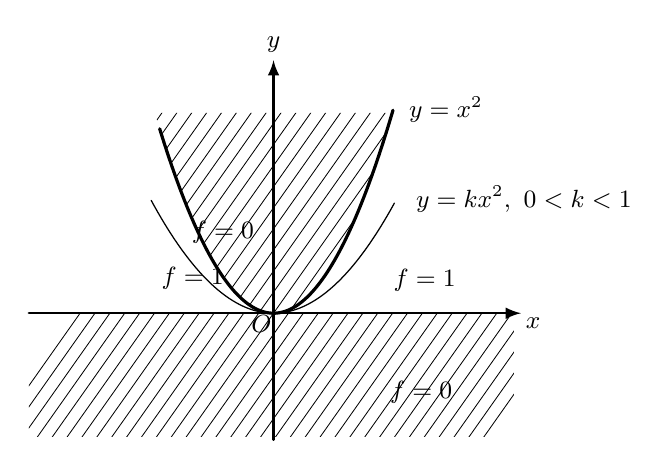
\begin{tikzpicture}[x=25.4pt, y=25.4pt, >=latex, line cap=round]
      % ---------- 上半阴影区域: y > x^2 (f = 0) ----------
      \begin{scope}
        \clip plot[domain=-1.688:1.688, samples=120] (\x, {\x*\x})
              -- (1.688, 2.85) -- (-1.688, 2.85) -- cycle;
        \foreach \c in {-6.0, -5.70, ..., 7.20} {
          \draw[line width=0.30pt] (-4.3, {1.417*(-4.3) + \c}) -- (4.3, {1.417*4.3 + \c});
        }
      \end{scope}
      % ---------- 下半阴影区域: y < 0 (f = 0) ----------
      \begin{scope}
        \clip (-3.48, -1.75) rectangle (3.42, 0);
        \foreach \c in {-6.0, -5.70, ..., 4.0} {
          \draw[line width=0.30pt] (-4.3, {1.417*(-4.3) + \c}) -- (4.3, {1.417*4.3 + \c});
        }
      \end{scope}
      % ---------- 坐标轴 ----------
      \draw[->, line width=0.9pt] (-3.48, 0) -- (3.52, 0) node[below right=-2pt] {\small $x$};
      \draw[->, line width=0.9pt] (0, -1.80) -- (0, 3.60) node[above=-1pt] {\small $y$};
      \node[below left=-1pt, inner sep=1.5pt] at (0, 0) {\small $O$};
      % ---------- 抛物线 y = x^2 (粗) 与 y = k x^2, 0<k<1 (细) ----------
      \draw[line width=1.15pt] plot[domain=-1.62:1.70, samples=120] (\x, {\x*\x});
      \draw[line width=0.45pt] plot[domain=-1.74:1.72, samples=120] (\x, {0.53*\x*\x});
      % ---------- 标注 ----------
      \node[inner sep=1pt] at (-1.15, 0.50) {\small $f = 1$};
      \node[inner sep=1pt] at (2.15, 0.47) {\small $f = 1$};
      \node[inner sep=1pt] at (-0.72, 1.15) {\small $f = 0$};
      \node[inner sep=1pt] at (2.10, -1.12) {\small $f = 0$};
      \node[anchor=west, inner sep=1pt] at (1.88, 2.90) {\small $y = x^{2}$};
      \node[anchor=west, inner sep=1pt] at (1.98, 1.62) {\small $y = kx^{2},\ 0 < k < 1$};
    \end{tikzpicture}
    \caption{}\label{fig:7.5.1}
  \end{figure}

  \item 证明:
  \[
    f(x, y) = \frac{1}{1 - xy}
  \]
  在 $D = [0, 1) \times [0, 1)$ 上连续, 但不一致连续.

  \item 设 $f(x, y)$ 定义在闭矩形 $[a, b] \times [c, d]$ 上. 如果 $f$ 对 $y$ 在 $[c, d]$ 上处处连续, 对 $x$ 在 $[a, b]$ (且关于 $y$!) 为一致连续. 证明: $f$ 在 $[a, b] \times [c, d]$ 上处处连续.

  \item (尤格定理) 设 $f$ 在 $\mathbb{R}^{2}$ 上分别对每一自变量 $x$ 与 $y$ 是连续的, 并且每当固定 $x$ 时 $f$ 对 $y$ 是单调的, 证明: $f$ 为 $\mathbb{R}^{2}$ 上的二元连续函数.

  \item 设 $\lim\limits_{y \to y_{0}} \varphi(y) = a$, $\lim\limits_{x \to x_{0}} \psi(x) = 0$, 且在 $(x_{0}, y_{0})$ 附近有 $|f(x, y) - \varphi(y)| \leqslant \psi(x)$. 证明:
  \[
    \lim_{(x, y) \to (x_{0}, y_{0})} f(x, y) = a.
  \]

  \item 设 $A$ 为 $(\mathbb{R}^{n}, \mathcal{T}_{\rho_{0}}^{n})$ 中的有界开集, $f\colon A \to \mathbb{R}$ 为一致连续的函数. 证明:

  \begin{tabular}{@{}p{0.45\linewidth}p{0.50\linewidth}@{}}
    (1) 可将 $f$ 延拓到 $\overline{A}$ 上; & (2) $f$ 在 $A$ 上有界.
  \end{tabular}

  \item 设 $u = \varphi(x, y)$ 与 $v = \psi(x, y)$ 在 $xy$ 平面中的点集 $A$ 上一致连续; $\varphi$ 与 $\psi$ 将点集 $A$ 映为 $uv$ 平面中的点集 $D$, $f(u, v)$ 在 $D$ 上一致连续. 证明: 复合函数 $f(\varphi(x, y), \psi(x, y))$ 在 $A$ 上一致连续.

  \item 设 $(\mathbb{R}^{n}, \mathcal{T}_{\rho_{0}}^{n})$ 为 $n$ 维 Euclid 空间, $f\colon \mathbb{R}^{n} \to \mathbb{R}^{1}$ 为连续函数, $\alpha \in \mathbb{R}$,
  \[
    E = \left\{x = (x_{1}, x_{2}, \cdots, x_{n}) \mid f(x) = f(x_{1}, x_{2}, \cdots, x_{n}) > \alpha\right\} \subset \mathbb{R}^{n},
  \]
  \[
    F = \left\{x = (x_{1}, x_{2}, \cdots, x_{n}) \mid f(x) = f(x_{1}, x_{2}, \cdots, x_{n}) \geqslant \alpha\right\} \subset \mathbb{R}^{n}.
  \]
  证明: $E$ 为 $(\mathbb{R}^{n}, \mathcal{T}_{\rho_{0}}^{n})$ 中的开集, $F$ 为 $(\mathbb{R}^{n}, \mathcal{T}_{\rho_{0}}^{n})$ 中的闭集.

  \item 设 $f(x, y) = \dfrac{1}{xy}$, $r = \sqrt{x^{2} + y^{2}}$, $k > 1$,
  \[
    D_{1} = \left\{(x, y)\ \middle|\ \frac{x}{k} \leqslant y \leqslant kx\right\},
  \]
  \[
    D_{2} = \{(x, y) \mid x > 0,\ y > 0\}.
  \]
  试分别讨论 $i = 1, 2$ 时极限 $\lim\limits_{\substack{(x, y) \in D_{i} \\ r \to +\infty}} f(x, y)$ 是否存在? 并说明理由.

  \item 设 $f(t)$ 在开区间 $(a, b)$ 内连续可导, 在开区间 $D = (a, b) \times (a, b)$ 内定义函数
  \[
    F(x, y) =
    \begin{cases}
      \dfrac{f(x) - f(y)}{x - y}, & x \neq y, \\[2.5mm]
      f'(x), & x = y.
    \end{cases}
  \]
  证明: $\forall c \in (a, b)$, 有 $\lim\limits_{(x, y) \to (c, c)} F(x, y) = f'(c)$.

  \item 设 $\varphi(x)$ 在 $[a, b]$ 上连续, 令 $f(x, y) = \varphi(x)$, $(x, y) \in D = [a, b] \times (-\infty, +\infty)$. 证明: $f$ 在 $D$ 上连续且为一致连续函数.

  \item 设 $f$ 在 $\mathbb{R}^{2}$ 上连续, 且 $\lim\limits_{r \to +\infty} f(x, y) = a$, $r = \sqrt{x^{2} + y^{2}}$. 证明:

  \begin{tabular}{@{}p{0.45\linewidth}p{0.50\linewidth}@{}}
    (1) $f$ 在 $\mathbb{R}^{2}$ 上有界; & (2) $f$ 在 $\mathbb{R}^{2}$ 上一致连续.
  \end{tabular}

  \item 叙述并证明二元函数的局部保号性.

  \item 设 $E$ 与 $F$ 为度量空间 $(X, \mathcal{T})$ 中的两个不相交的闭集. 证明:
  (1) $U_{E} = \{x \mid \rho(x, E) < \rho(x, F)\} \subset X$ 与 $U_{F} = \{x \mid \rho(x, E) > \rho(x, F)\} \subset X$ 分别为 $E$ 与 $F$ 的两个不相交的开邻域;
  (2) $U_{E} = \bigcup\limits_{x \in E} B\left(x; \dfrac{1}{3}\rho(x, F)\right)$ 与 $U_{F} = \bigcup\limits_{x \in F} B\left(x; \dfrac{1}{3}\rho(x, E)\right)$ 分别为 $E$ 与 $F$ 的两个不相交的开邻域.

  \item 设 $(X, \rho)$ 为度量空间, $A \neq \varnothing$ 且 $A \subset X$, 则 $f\colon X \to \mathbb{R}$, $f(x) = \rho(x, A)$ 为 $X$ 上的一致连续函数.

  \item 设函数 $f(x, y)$ 在 $[a, A] \times [b, B]$ 上连续, 而函数列 $\{\varphi_{n}(x)\}$ 在 $[a, A]$ 上一致收敛, 且 $b \leqslant \varphi_{n}(x) \leqslant B$, $n \in \mathbb{Z}_{+}$. 证明: 函数列 $\{F_{n}(x)\} = \{f(x, \varphi_{n}(x))\}$ 也在 $[a, A]$ 上一致收敛.

  \item 设 (1) 函数 $f(x, y)$ 于 $(a, A) \times (b, B)$ 内是连续的; (2) 函数 $\varphi(x)$ 于区间 $(a, A)$ 内连续且 $b < \varphi(x) < B$. 证明: 函数
  \[
    F(x) = f(x, \varphi(x))
  \]
  在区间 $(a, A)$ 内是连续的.

  \item 设 (1) 函数 $f(x, y)$ 于 $(a, A) \times (b, B)$ 内是连续的; (2) 函数 $x = \varphi(u, v)$, $y = \psi(u, v)$ 在 $(a', A') \times (b', B')$ 内是连续的, 并分别有属于 $(a, A)$ 与 $(b, B)$ 的值. 证明: 函数
  \[
    F(u, v) = f(\varphi(u, v), \psi(u, v))
  \]
  在 $(a', A')$ 内连续.

  \item 设 $(u, v) = F(x, y) = (f(x, y), g(x, y))$, 其中
  \[
    u = f(x, y) =
    \begin{cases}
      \dfrac{x}{(x^{2} + y^{2})^{\alpha}}\ln(|x| + |y|), & x^{2} + y^{2} \neq 0, \\[2.5mm]
      0, & x^{2} + y^{2} = 0;
    \end{cases}
  \]
  \[
    v = g(x, y) =
    \begin{cases}
      \dfrac{y}{(x^{2} + y^{2})^{\alpha}}\ln(|x| + |y|), & x^{2} + y^{2} \neq 0, \\[2.5mm]
      0, & x^{2} + y^{2} = 0.
    \end{cases}
  \]
  讨论 $F(x, y)$ 的连续性.
\end{exblock}
